\chapter{Implementation}
The following chapter will outline the implementation process and how the project was developed. Firstly, an overview of the dataset used shall be given with information on how the images were preprocessed and augmented for training. A section for the model implementation will be given to describe how the convolutional neural network (CNN) was developed using Tensorflow. This is followed by the deployment process of the Tensorflow Python API. Lastly, the steps in which the Node.JS web application was made shall be touched upon, accompanied by the design and features choices.

\section{Data Understanding}
As stated in the system design, the dataset that will be used is the Cohn-Kanade+ image dataset, which release in 2000 with the purpose of classifying facial expressions \citep{ck}. The dataset consists of images of 210 subject between the ages of 18 and 50. Each subject is asked to show a a facial expression, beginning with a neutral facial expression that eventually lapses to the target emotion. The digital images come in either a 640x490 or 640x480 pixel format. Furthermore, the images either consists of an 8-bit grayscale or 24-bit colour format \citep{ck}. The dataset is made up of 593 image sequences and provides labels for each sequence, ranging between 0 and 6. Refer to Figure \ref{seq} for a summarized illustration of how these sequences are built.

\begin{figure}[ht]
	\begin{center}
		\advance\leftskip-3cm
		\advance\rightskip-3cm
		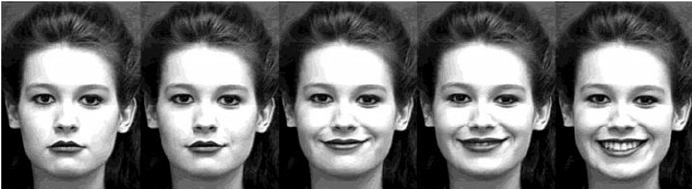
\includegraphics[keepaspectratio=true,scale=0.6]{__resources/DATASET/sequence.png}
		\caption{Image Sequence From Neutral to Happy}
		\label{seq}
	\end{center}
\end{figure}

It should be noted that the figure above is not a full image sequence and the some transitional images have been omitted. Moreover, it should also be known that there are inconsistencies in the dataset, such as many subject not having image sequences for each certain emotions and label data missing for some images. This is acknowledged in the \textit{README} file created by Lucey et al. that is contained within the dataset, where it is declared "\textit{IF THERE IS NO FILE IT MEANS THAT THERE IS NO EMOTION LABEL (sorry to be explicit but this will avoid confusion)}". 

\section{Data Preparation and Preprocessing}
A number of preprocessing steps were taken in order to prepare the images for training the network. These steps were required to ensure maximum possible accuracy and minimal training time as the nature of working with neural networks can be computationally expensive when accompanied with large files such as images. The steps are as follows: Image extraction, Gray scaling, Facial Cropping, Data Augmentation and Data Splitting.

\subsection{Image Extraction}
Due to the structure of the image sequence within the datasets, it is undesirable to used all images within each sequence as that do accurately resemble the facial expression it is used to represent. Therefore, for each sequence the last four images were extracted from their directory and relocated to a new directory under the category of facial expression they represent. As stated in the system design, images for disgust and contempt are omitted from this new dataset. Furthermore, because there is now class for a neutral facial expression, the first four images from a sequence in each subject was extracted.

\subsection{Gray Scaling}
The CK+ dataset consist of a majority of gray images. However, the extended version of this dataset contains some images sequences with coloured images. When working neural networks, it is significantly more computationally expensive to process a coloured image over a gray one due to the number of colour channels. To mitigate this, a Python script was created to traverse through each image of the newly extracted dataset to convert all images to grayscale using the PILLOW library. \\

\begin{lstlisting}[language=Python, frame=single]
from PIL import Image
import numpy as np
import os, os.path
img_path = '<DATASET_DIRECTORY>' 

def grayify(file_name):
	image = Image.open(img_path + file_name)
	image = image.convert('L')
	image.save(img_path + file_name)

#Load the directory and traverse over all the image files
list = os.listdir(img_path)
for file in list:
	file_n = file
	print(file_n)

\end{lstlisting}

\subsection{Facial Cropping}
Following the gray scaling of all images, dimensionality reduction was implemented on the images. This was done by cropping each image down to only the facial surface area. This is done to reduce the noise of the data and to remove any features in the backgrounds that may be learned by the network that do not represent the facial expression. To do this, a Python script was written that reads in all the images from the dataset and crop the region of the image that contains the subject faces. This was done using the OpenCV library.

\begin{lstlisting}[language=Python, frame=single]
def facecrop(image):
	face_cascade = cv2.CascadeClassifier
	('haarcascade_frontalface_default.xml')
	
	img = cv2.imread(image)
	minisize = (img.shape[1],img.shape[0])
	miniframe = cv2.resize(img, minisize)
	faces = face_cascade.detectMultiScale(miniframe)
	
	for f in faces:
		x, y, w, h = [ v for v in f ]
		cv2.rectangle(img, (x,y), (x+w,y+h),
		(255,255,255))
		sub_face = img[y:y+h, x:x+w]
		fname, ext = os.path.splitext(image)
		cv2.imwrite(fname+"_cropped_"+ext, sub_face)
	return

list = os.listdir(<DIRECTORY_NAME>)
for file in list:
	facecrop(<DIRECTORY_NAME> + '/' + file)
\end{lstlisting}
\newpage
This was done for all images, however, some images were not correctly cropped due to noise in the image causing it to misclassify the facial region. Some examples of this might be only half the face being cropped into the new image or just the subjects shoulder being visible. These worthless images were manually deleted after the newly cropped images were evaluated. Please refer to Figure \ref{crop}for example of the facial cropping.

\begin{figure}[ht]
	\begin{center}
		\advance\leftskip-3cm
		\advance\rightskip-3cm
		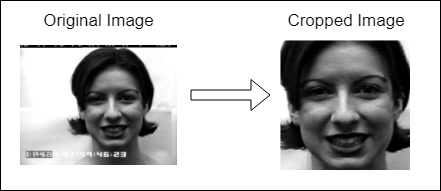
\includegraphics[keepaspectratio=true,scale=0.9]{__resources/DATASET/crop.png}
		\caption{Image Cropping on Facial Regions}
		\label{crop}
	\end{center}
\end{figure}
\newpage


\subsection{Image Increasing Through Data Augmentation}
Upon inspection of the dataset, in regards to the number of images for certain facial expressions, it was noted that there was an insufficient amount of images to train the network. This can be seen in table \ref{table: count}. 
\begin{table}
	\begin{tabular}{ |p{10cm}||p{3cm}|}
		\hline
		\textbf{Facial Expression} & \textbf{Cardinality}\\
		\hline
		\hline
		Anger & 601 \\
		\hline
		Fear & 427	\\
		\hline
		Happy & 883\\
		\hline
		Neutral & 668\\
		\hline
		Sad & 641	\\
		\hline
		Surprise  & 639	\\
		\hline
		\textbf{Total}  & \textbf{3879}	\\
		\hline
	\end{tabular}
	\caption{Initial Image Count}
	\label{table: count}
\end{table}

The initial step to increase the size of the data set was to flipped versions of all the images. Not only does this double the size of the dataset, but helps the network to better handle facial variance when dealing with new unseen data. Also, it will decrease the chance of under-fitting while training the model. Following this step, a check was done on the class balance. Using the Matplotlib Python library, the balance of each class was plotted by counting each image in accordance to it's respective label, as seen in Figure \ref{imbal}

\begin{figure}[ht]
	\begin{center}
		\advance\leftskip-3cm
		\advance\rightskip-3cm
		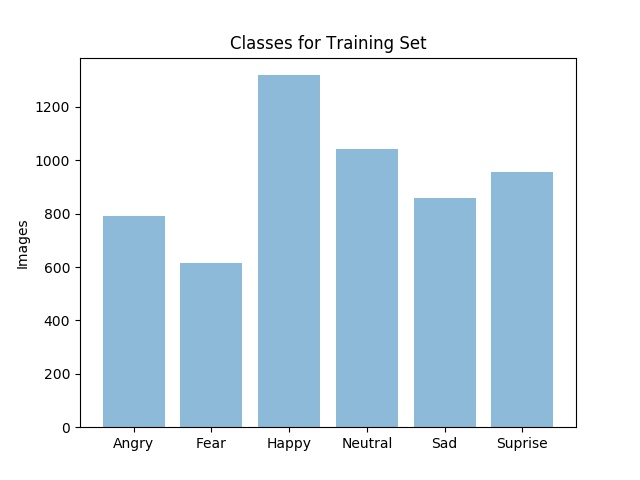
\includegraphics[keepaspectratio=true,scale=0.6]{__resources/implementation/imbalance.jpg}
		\caption{Class Imbalance}
		\label{imbal}
	\end{center}
\end{figure}\newpage
As seen above, expression 'Anger' and 'Fear' are under represented while 'Happy' is overly represented, relative to the rest of the dataset. How this problem was addressed was to create synthetic sample images from the existing ones by the means of skewing and augmenting the images. This can be seen in Figure \ref{augm}, where the top row displays the original cropped images. Beneath, are the slightly skewing images. This was implemented using a Python library called Augmentor, which allows you to specify the directory and number of altered samples you would like, and it randomly picks images within the directory, creating an entirely new back of images that have been stretched to a degree.
\begin{figure}[ht]
	\begin{center}
		\advance\leftskip-3cm
		\advance\rightskip-3cm
		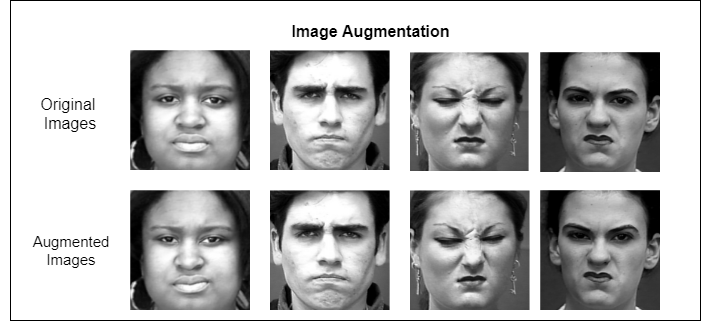
\includegraphics[keepaspectratio=true,scale=0.6]{__resources/implementation/augmented-images.png}
		\caption{Example of Augmented Images}
		\label{augm}
	\end{center}
\end{figure}
\newpage

This was done for all classes to increase the number of samples in the dataset, until a number of 1750 images are present for each class. This amounts to a total number of 10500 images in total across the entire dataset.  The class balance can be seen in the bar chart illustration in Figure \ref{bal}, which has been plotted using the Matplotlib library. In conclusion, an additional 6,621 images have been created from the original dataset.


\begin{figure}[ht]
	\begin{center}
		\advance\leftskip-3cm
		\advance\rightskip-3cm
		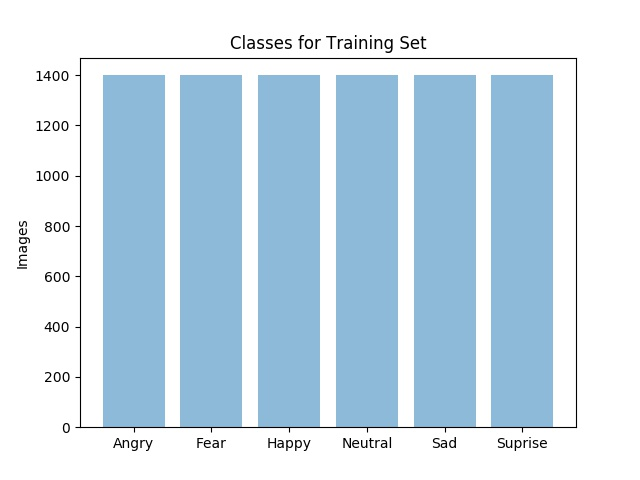
\includegraphics[keepaspectratio=true,scale=0.6]{__resources/implementation/balance.jpg}
		\caption{Class Balance}
		\label{bal}
	\end{center}
\end{figure}

\newpage

% show bad imbalance 
%flipping + synthethic examples
% show balance
\subsection{Data Splitting}
The last step in the the preparation phase was to apply split validation to the dataset. The dataset was split into training and testings sets at a divide of 80/20 - meaning 80\% of the dataset will be used for training (1400 images per class) and 20\% will be used for testing the model (350 images per class). Please see the Python code below showing how this was achieved.

\begin{lstlisting}[language=Python, frame=single]
import os, os.path
import math
from PIL import Image

old_path = 'C:/Users/aaron/Desktop/Cropped Dataset/happy/'

new_train_path ='C:/Users/aaron/Desktop/data/training/happy/'
new_test_path = 'C:/Users/aaron/Desktop/data/testing/happy/'

#Load the directory and traverse over all the image files
list = os.listdir(old_path)

# define the size of the first 80 percent of images
num_files = len(list)
num_training_files = num_files * .8
num_training_files = math.ceil(num_training_files)

num_testing_file = num_files * .2
num_testing_file = math.ceil(num_testing_file)

#Add the first 80 percent to the training folder
for img in list[1:num_training_files]: 
	i = Image.open(old_path + img)
	i.save(new_train_path+img)


#Add the remaining 20 percent to the training folder
for img in list[num_training_files:]:
	i = Image.open(old_path + img)
	i.save(new_test_path+img)
\end{lstlisting}

\section{Implementing the Machine Learning Model}

When implementing the machine learning model with Tensorflow, the initial step used is to import all the libraries that deemed necessary for preprocessing and training. These include Tensorflow, Numpy, Skimage and the os packages. Secondly, the image data was import with it's respective labels. A lists are used to store the image RGB data for every image in the dataset. This means we have a list of lists in our program. Secondly, for each image in a directory under a certain class, a label of that class is added to the labels list. Refer code below to see how this was implemented.

\begin{lstlisting}[language=Python, frame=single]
def load_data(TRAINING_DIR):
images = []
labels = []

directories = [d for d in os.listdir(TRAINING_DIR) 
if os.path.isdir(os.path.join(TRAINING_DIR, d))]

# Traverse through each directory and make a list
# of files names if they end in the PNG format
for d in directories:
	label_directory = os.path.join(TRAINING_DIR, d)
	file_names = [os.path.join(label_directory, f) 
	for f in os.listdir(label_directory) 
				if f.endswith(".png")]
	
	#Traverse through each file, add the image data
	# and label to the 2 lists
	for f in file_names:
		images.append(skimage.data.imread(f))
		labels.append(int(d))
	return images, labels

images, labels = load_data(TRAINING_DIR)
\end{lstlisting}


Following the importation of the images and labels, some further preprocessing steps are done. In this case, each image in the list of images are sub sampled from their original sizes down to a 50x50 pixel size. This was done to reduce the dimensionality of the images for the network to better handle the input data. This was done using the \textbf{Skimage} library. The list images were traversed and resized using the tranform function. 
\begin{lstlisting}[frame=single]
images = [transform.resize(image,(50, 50))
	for image in images]
\end{lstlisting}
After basic data imports, defining the computation graph for Tensorflow is required.
Tensorflow placeholder were then declared for later use when tensors need to be fed to the Tensorflow session, along with another few initial variables such as number of epochs, the batch size, dropout rate etc.  After this, the structure of the network was defined. 
The network consists of 3 convolution layers with an activation function of Relu, 3 max-pooling. The input from the image value is multiplied by the random weight assigned to each node, and the bias is added (both of which are have been defined in Python dictionaries). This structure is done for all 3 convolution/max-pooling layers, as seen in Figure \ref{map}.

\begin{figure}[ht]
	\begin{center}
		\advance\leftskip-3cm
		\advance\rightskip-3cm
		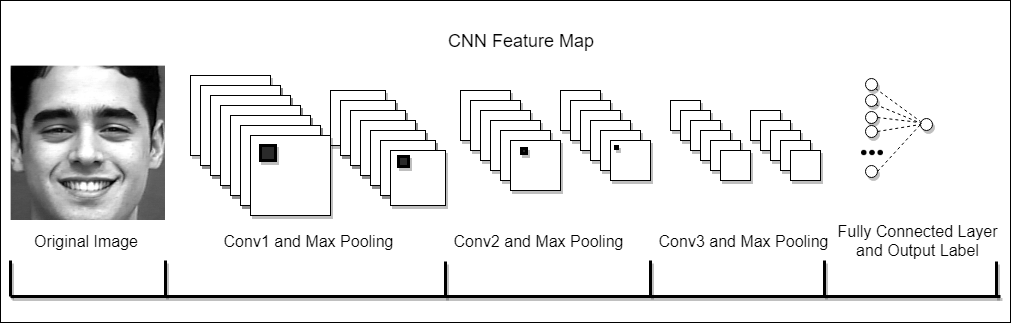
\includegraphics[keepaspectratio=true,scale=0.5]{__resources/implementation/map.png}
		\caption{Feature Map of CNN}
		\label{map}
	\end{center}
\end{figure}
Lastly, a fully connected layer is defined, which will be used to produce a predicted output.The reason dropout is used in this case is to reduce the chances of over fitting the network. After each training iteration (epoch), only 80 percent of the trained neurons are kept.\\ \\



\begin{lstlisting}[language=python, frame=single]
conv1 = tf.nn.relu(conv2d(x, weights['weights_conv1'])
		 + biases['bias_conv1'])
conv1 = maxpool2d(conv1)

conv2 = tf.nn.relu(conv2d(conv1, weights['weights_conv2'])
		 + biases['bias_conv2'])
conv2 = maxpool2d(conv2)

conv3 = tf.nn.relu(conv2d(conv2, weights['weights_conv3']) 
		+ biases['bias_conv3'])
conv3 = maxpool2d(conv3)

fully_con = tf.reshape(conv3, [-1, 7*7*256])
fully_con = tf.nn.relu(tf.matmul(fully_con,
	 weights['weights_fully_con'])
 	 + biases['bias_fully_con'])
 
fc = tf.nn.dropout(fully_con, keep_rate) # Apply dropout

output = tf.matmul(fully_con, weights['weights_out']) 
		+ biases['bias_out']
return output
\end{lstlisting}

Following the structure set up of the network, a function is defined that runs the Tensorflow session, which takes the \textbf{x} placeholder as a parameter. The session is ran by first initializing all the Tensorflow variables, then iterated through
the number of epochs and feed the image data and labels using feed\_dict.
The loss/cost and accuracy is evaluated and printed to the console.\\

\begin{lstlisting}[language=python, frame=single]
def train_network(x):
  saver = tf.train.Saver()
  pred = convolutional_network(x)
  loss = tf.reduce_mean(
  tf.nn.sparse_softmax_cross_entropy_with_logits(labels
   = y, logits = pred))
 
  train_op = tf.train.AdamOptimizer(learning_rate=0.01)
          .minimize(loss)

  with tf.Session() as sess:
	# Initialize all the variables
	sess.run(tf.global_variables_initializer())

  print("RUNNING SESSION...")
  for epoch in range(num_epochs):
    _, loss_value = sess.run([train_op, loss], 
               feed_dict={x: images, y: labels})
                   
  print('Epoch:', epoch+1, "of", num_epochs, '-Loss:',
  		 loss_value)
  	....
\end{lstlisting}

% Image images
% preprocessing
% Create comptation graph
% create session

\section{Deploying the Trained Model}
% 1 - Flask API

\section{Implementing the Node.JS Application}
To develop a web application for the user to interact with, Node.JS was used to implement a simple one page application that accesses the users webcam. Firstly, a javascript webserver was created using the Express npm module, which provides functions for routing and serving html pages. A port is initially set using either port 5000 for local development, or a randomly allocated port for deployment. 

\begin{lstlisting}[language=python, frame=single]
	app.set('port', (process.env.PORT || 5000))
\end{lstlisting}

This is followed by providing the home page when the base route is called by from the client. When the \textbf{'/'} route is called, a html page containing the application is delivered to the users browser and displayed in the DOM.

\begin{lstlisting}[language=python, frame=single]
app.get('/', function (req, res) {
  res.sendFile(path.join(__dirname, '/index.html'));
});

var server = app.listen(app.get('port'), function () {
  var host = server.address().address
  console.log('Application running on port', app.get('port'))
})
\end{lstlisting}

\subsection{Facial Tracking With a Users Webcam}

The user interface design of the application is very simple. On the left hand side a the page the webcam feed is displayed. This accesses the user's machine's webcam and displays it to the screen using the html \textbf{canvas} element. Canvas is a container for drawing graphics to the page. For facial tracking, a library called Tracking.js was imported. Trackin.js is an open source library created by Eduardo Lundgren for object, colour and face detection using javascript. The reason for this library choice was because other alternatives, such as OpenCV, deemed to be very heavy weight in comparison and API services that have also been considered such as cloudinary would reduce classification speed as it would be computationally expressive to make multiple requests for facial cropping while using the application. 
In light of this, tracking.js provides a lightweight and quick solution for detecting faces. Using what is known as haar cascades, object classification and detection is made simplified and provides fast calculation speeds. In terms of the web application, the canvas drawing of the webcam feed is read and interpreted by tracking.js and the facial features are detected. A yellow box is drawn around the detected facial area.
\begin{lstlisting}[language=python, frame=single]
var tracker = new tracking.ObjectTracker('face');
tracker.setInitialScale(4);
tracker.setStepSize(.5);
tracker.setEdgesDensity(0.1);
tracking.track('#video', tracker, { camera: true });
tracker.on('track', function(event) {
context.clearRect(0, 0, canvas.width, canvas.height);
\end{lstlisting}

One function that tracking.js does not provide is the ability to crop the detected area of the stream. To get around this, java script code was developed to mark the area in which the square was being drawn around the users face. In each frame of a users face being detected a new square is drawn to the canvas, so every time that a new square is displayed to the screen, this marks the new coordinates of the area in which is needed for cropping. 

\begin{lstlisting}[language=python, frame=single]
rect_width = rect.width; // 
rect_height = rect.height;
rectX = rect.x;
rectY = rect.y;

 ...

ctx.drawImage(video, rectX+ 100, rectY +90,
	 rect_width +70,  rect_height +50, 0, 0, 300, 150);
\end{lstlisting}

After is is known where the users face is positioned in the shot, the cropped area is displayed in a separate 100x100 pixel canvas area, named ctx, below the feed. To ensure that the trained Tensorflow API does not become overflowed with image data, an interval timing is implemented. This involves setting a timer as to when an image is cropped because it would be disadvantageous and computationally expensive to have every frame to be sent to the API. In this case, the interval is set to 1 second. To initiate a session with the model and begin the facial sentiment analysis, a button was added to the UI which begins the analysis. Please refer to the Figure \ref{web} for a screenshot of the facial tracking in action.

\begin{figure}[ht]
	\begin{center}
		\advance\leftskip-3cm
		\advance\rightskip-3cm
		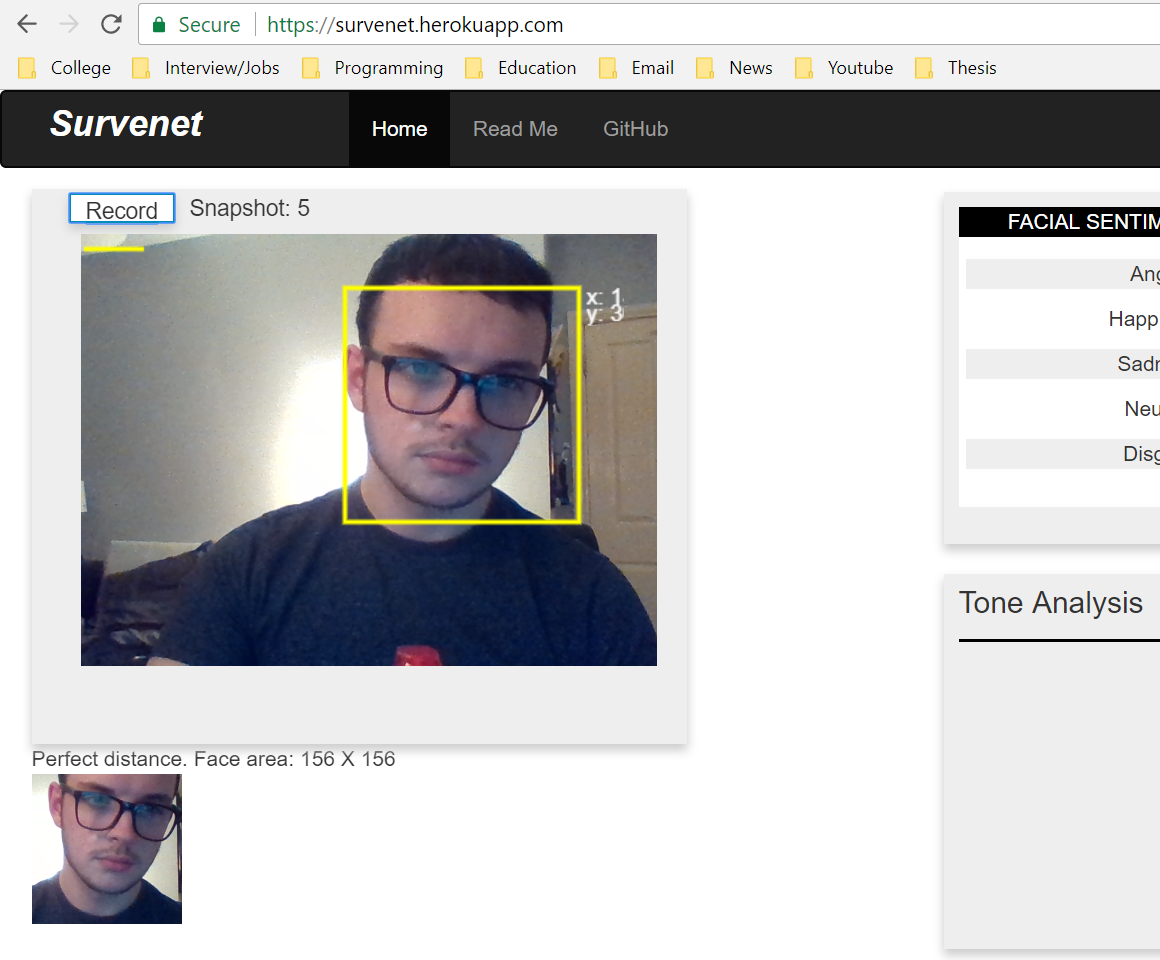
\includegraphics[keepaspectratio=true,scale=0.5]{__resources/implementation/webapp1.png}
		\caption{Webcam Feed with Facial Tracking and Cropping}
		\label{web}
	\end{center}
\end{figure}


\subsection{Facial Sentiment Analysis} 

% 1 - Create Node/express application
% 2 - Implement webcam canvas
% 3 - Apply tracking.js
% 4 - impelement facial cropping
% 5 - Make request to API

\section{Deploying the Node.JS Application}
% 1 - Github
% 2 - Heroku integration




%\subsection{Database Integration

%\section{Result Weighting Algorithm}

%\section{Integrating Third Party Services}

\section{Concluding Remarks of Implementation}
